% Created by tikzDevice version 0.12 on 2018-09-28 04:17:12
% !TEX encoding = UTF-8 Unicode
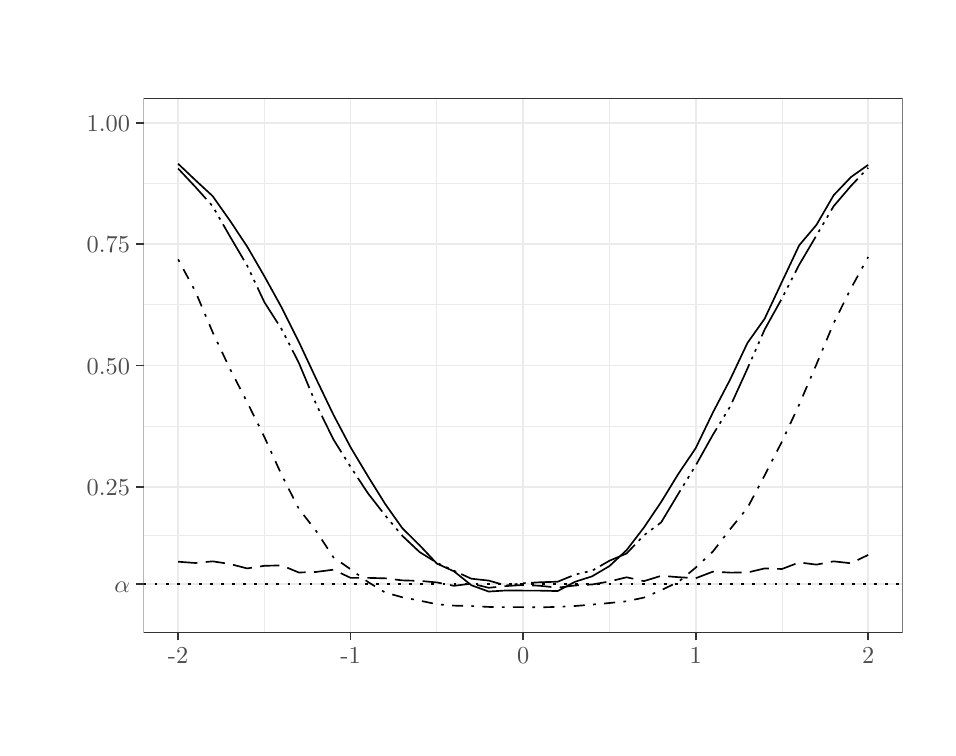
\begin{tikzpicture}[x=1pt,y=1pt]
\definecolor{fillColor}{RGB}{255,255,255}
\path[use as bounding box,fill=fillColor,fill opacity=0.00] (0,0) rectangle (325.21,252.94);
\begin{scope}
\path[clip] (  0.00,  0.00) rectangle (325.21,252.94);
\definecolor{drawColor}{RGB}{255,255,255}
\definecolor{fillColor}{RGB}{255,255,255}

\path[draw=drawColor,line width= 0.6pt,line join=round,line cap=round,fill=fillColor] (  0.00,  0.00) rectangle (325.21,252.94);
\end{scope}
\begin{scope}
\path[clip] ( 41.90, 34.26) rectangle (316.18,227.38);
\definecolor{fillColor}{RGB}{255,255,255}

\path[fill=fillColor] ( 41.90, 34.26) rectangle (316.18,227.38);
\definecolor{drawColor}{gray}{0.92}

\path[draw=drawColor,line width= 0.3pt,line join=round] ( 41.90, 69.37) --
	(316.18, 69.37);

\path[draw=drawColor,line width= 0.3pt,line join=round] ( 41.90,108.87) --
	(316.18,108.87);

\path[draw=drawColor,line width= 0.3pt,line join=round] ( 41.90,152.76) --
	(316.18,152.76);

\path[draw=drawColor,line width= 0.3pt,line join=round] ( 41.90,196.65) --
	(316.18,196.65);

\path[draw=drawColor,line width= 0.3pt,line join=round] ( 85.53, 34.26) --
	( 85.53,227.38);

\path[draw=drawColor,line width= 0.3pt,line join=round] (147.87, 34.26) --
	(147.87,227.38);

\path[draw=drawColor,line width= 0.3pt,line join=round] (210.21, 34.26) --
	(210.21,227.38);

\path[draw=drawColor,line width= 0.3pt,line join=round] (272.55, 34.26) --
	(272.55,227.38);

\path[draw=drawColor,line width= 0.6pt,line join=round] ( 41.90, 51.81) --
	(316.18, 51.81);

\path[draw=drawColor,line width= 0.6pt,line join=round] ( 41.90, 86.93) --
	(316.18, 86.93);

\path[draw=drawColor,line width= 0.6pt,line join=round] ( 41.90,130.82) --
	(316.18,130.82);

\path[draw=drawColor,line width= 0.6pt,line join=round] ( 41.90,174.71) --
	(316.18,174.71);

\path[draw=drawColor,line width= 0.6pt,line join=round] ( 41.90,218.60) --
	(316.18,218.60);

\path[draw=drawColor,line width= 0.6pt,line join=round] ( 54.37, 34.26) --
	( 54.37,227.38);

\path[draw=drawColor,line width= 0.6pt,line join=round] (116.70, 34.26) --
	(116.70,227.38);

\path[draw=drawColor,line width= 0.6pt,line join=round] (179.04, 34.26) --
	(179.04,227.38);

\path[draw=drawColor,line width= 0.6pt,line join=round] (241.38, 34.26) --
	(241.38,227.38);

\path[draw=drawColor,line width= 0.6pt,line join=round] (303.71, 34.26) --
	(303.71,227.38);
\definecolor{drawColor}{RGB}{0,0,0}

\path[draw=drawColor,line width= 0.6pt,dash pattern=on 1pt off 3pt on 4pt off 3pt ,line join=round] ( 54.37,169.20) --
	( 60.60,157.61) --
	( 66.83,142.93) --
	( 73.07,129.69) --
	( 79.30,117.65) --
	( 85.53,105.04) --
	( 91.77, 91.32) --
	( 98.00, 79.06) --
	(104.24, 71.06) --
	(110.47, 61.58) --
	(116.70, 57.22) --
	(122.94, 52.66) --
	(129.17, 48.83) --
	(135.40, 47.11) --
	(141.64, 45.92) --
	(147.87, 44.58) --
	(154.10, 44.09) --
	(160.34, 43.95) --
	(166.57, 43.63) --
	(172.81, 43.53) --
	(179.04, 43.56) --
	(185.27, 43.49) --
	(191.51, 43.63) --
	(197.74, 43.95) --
	(203.97, 44.48) --
	(210.21, 45.04) --
	(216.44, 45.67) --
	(222.68, 47.00) --
	(228.91, 49.67) --
	(235.14, 52.66) --
	(241.38, 57.82) --
	(247.61, 63.65) --
	(253.84, 71.72) --
	(260.08, 79.41) --
	(266.31, 91.18) --
	(272.55,103.36) --
	(278.78,116.74) --
	(285.01,131.27) --
	(291.25,146.20) --
	(297.48,158.70) --
	(303.71,170.07);

\path[draw=drawColor,line width= 0.6pt,dash pattern=on 15pt off 2pt on 1pt off 2pt on 1pt off 2pt on 1pt off 2pt ,line join=round] ( 54.37,202.03) --
	( 60.60,195.39) --
	( 66.83,188.44) --
	( 73.07,177.55) --
	( 79.30,166.98) --
	( 85.53,153.75) --
	( 91.77,143.98) --
	( 98.00,131.80) --
	(104.24,116.88) --
	(110.47,104.17) --
	(116.70, 94.20) --
	(122.94, 84.71) --
	(129.17, 76.71) --
	(135.40, 69.30) --
	(141.64, 63.44) --
	(147.87, 59.57) --
	(154.10, 56.66) --
	(160.34, 53.82) --
	(166.57, 53.15) --
	(172.81, 51.36) --
	(179.04, 52.20) --
	(185.27, 52.55) --
	(191.51, 52.73) --
	(197.74, 55.29) --
	(203.97, 56.73) --
	(210.21, 60.31) --
	(216.44, 62.95) --
	(222.68, 69.51) --
	(228.91, 74.18) --
	(235.14, 84.57) --
	(241.38, 94.72) --
	(247.61,105.85) --
	(253.84,116.03) --
	(260.08,129.73) --
	(266.31,143.88) --
	(272.55,155.11) --
	(278.78,167.26) --
	(285.01,177.83) --
	(291.25,188.44) --
	(297.48,195.74) --
	(303.71,202.31);

\path[draw=drawColor,line width= 0.6pt,dash pattern=on 7pt off 3pt ,line join=round] ( 54.37, 59.96) --
	( 60.60, 59.50) --
	( 66.83, 60.10) --
	( 73.07, 59.15) --
	( 79.30, 57.54) --
	( 85.53, 58.49) --
	( 91.77, 58.63) --
	( 98.00, 56.06) --
	(104.24, 56.27) --
	(110.47, 57.08) --
	(116.70, 54.13) --
	(122.94, 54.13) --
	(129.17, 53.96) --
	(135.40, 53.22) --
	(141.64, 53.04) --
	(147.87, 52.48) --
	(154.10, 51.25) --
	(160.34, 52.06) --
	(166.57, 50.55) --
	(172.81, 51.15) --
	(179.04, 51.57) --
	(185.27, 51.25) --
	(191.51, 50.59) --
	(197.74, 51.36) --
	(203.97, 51.74) --
	(210.21, 52.83) --
	(216.44, 54.34) --
	(222.68, 52.94) --
	(228.91, 54.87) --
	(235.14, 54.38) --
	(241.38, 53.99) --
	(247.61, 56.38) --
	(253.84, 56.03) --
	(260.08, 56.06) --
	(266.31, 57.54) --
	(272.55, 57.33) --
	(278.78, 59.71) --
	(285.01, 58.91) --
	(291.25, 60.10) --
	(297.48, 59.40) --
	(303.71, 62.42);

\path[draw=drawColor,line width= 0.6pt,line join=round] ( 54.37,203.75) --
	( 60.60,197.85) --
	( 66.83,192.09) --
	( 73.07,183.24) --
	( 79.30,173.86) --
	( 85.53,163.12) --
	( 91.77,151.81) --
	( 98.00,139.38) --
	(104.24,126.04) --
	(110.47,113.09) --
	(116.70,101.29) --
	(122.94, 90.86) --
	(129.17, 80.85) --
	(135.40, 72.04) --
	(141.64, 65.89) --
	(147.87, 59.29) --
	(154.10, 56.45) --
	(160.34, 51.46) --
	(166.57, 49.18) --
	(172.81, 49.57) --
	(179.04, 49.53) --
	(185.27, 49.50) --
	(191.51, 49.36) --
	(197.74, 52.69) --
	(203.97, 54.69) --
	(210.21, 58.38) --
	(216.44, 64.17) --
	(222.68, 72.32) --
	(228.91, 81.55) --
	(235.14, 91.74) --
	(241.38,100.97) --
	(247.61,113.89) --
	(253.84,125.80) --
	(260.08,139.00) --
	(266.31,147.78) --
	(272.55,161.08) --
	(278.78,174.29) --
	(285.01,181.66) --
	(291.25,192.40) --
	(297.48,198.94) --
	(303.71,203.36);

\path[draw=drawColor,line width= 0.6pt,dash pattern=on 1pt off 3pt ,line join=round] ( 41.90, 51.81) -- (316.18, 51.81);
\definecolor{drawColor}{gray}{0.20}

\path[draw=drawColor,line width= 0.6pt,line join=round,line cap=round] ( 41.90, 34.26) rectangle (316.18,227.38);
\end{scope}
\begin{scope}
\path[clip] (  0.00,  0.00) rectangle (325.21,252.94);
\definecolor{drawColor}{gray}{0.30}

\node[text=drawColor,anchor=base east,inner sep=0pt, outer sep=0pt, scale=  0.88] at ( 36.95, 48.78) {$\alpha$};

\node[text=drawColor,anchor=base east,inner sep=0pt, outer sep=0pt, scale=  0.88] at ( 36.95, 83.90) {$0.25$};

\node[text=drawColor,anchor=base east,inner sep=0pt, outer sep=0pt, scale=  0.88] at ( 36.95,127.79) {$0.50$};

\node[text=drawColor,anchor=base east,inner sep=0pt, outer sep=0pt, scale=  0.88] at ( 36.95,171.68) {$0.75$};

\node[text=drawColor,anchor=base east,inner sep=0pt, outer sep=0pt, scale=  0.88] at ( 36.95,215.57) {$1.00$};
\end{scope}
\begin{scope}
\path[clip] (  0.00,  0.00) rectangle (325.21,252.94);
\definecolor{drawColor}{gray}{0.20}

\path[draw=drawColor,line width= 0.6pt,line join=round] ( 39.15, 51.81) --
	( 41.90, 51.81);

\path[draw=drawColor,line width= 0.6pt,line join=round] ( 39.15, 86.93) --
	( 41.90, 86.93);

\path[draw=drawColor,line width= 0.6pt,line join=round] ( 39.15,130.82) --
	( 41.90,130.82);

\path[draw=drawColor,line width= 0.6pt,line join=round] ( 39.15,174.71) --
	( 41.90,174.71);

\path[draw=drawColor,line width= 0.6pt,line join=round] ( 39.15,218.60) --
	( 41.90,218.60);
\end{scope}
\begin{scope}
\path[clip] (  0.00,  0.00) rectangle (325.21,252.94);
\definecolor{drawColor}{gray}{0.20}

\path[draw=drawColor,line width= 0.6pt,line join=round] ( 54.37, 31.51) --
	( 54.37, 34.26);

\path[draw=drawColor,line width= 0.6pt,line join=round] (116.70, 31.51) --
	(116.70, 34.26);

\path[draw=drawColor,line width= 0.6pt,line join=round] (179.04, 31.51) --
	(179.04, 34.26);

\path[draw=drawColor,line width= 0.6pt,line join=round] (241.38, 31.51) --
	(241.38, 34.26);

\path[draw=drawColor,line width= 0.6pt,line join=round] (303.71, 31.51) --
	(303.71, 34.26);
\end{scope}
\begin{scope}
\path[clip] (  0.00,  0.00) rectangle (325.21,252.94);
\definecolor{drawColor}{gray}{0.30}

\node[text=drawColor,anchor=base,inner sep=0pt, outer sep=0pt, scale=  0.88] at ( 54.37, 23.25) {-2};

\node[text=drawColor,anchor=base,inner sep=0pt, outer sep=0pt, scale=  0.88] at (116.70, 23.25) {-1};

\node[text=drawColor,anchor=base,inner sep=0pt, outer sep=0pt, scale=  0.88] at (179.04, 23.25) {0};

\node[text=drawColor,anchor=base,inner sep=0pt, outer sep=0pt, scale=  0.88] at (241.38, 23.25) {1};

\node[text=drawColor,anchor=base,inner sep=0pt, outer sep=0pt, scale=  0.88] at (303.71, 23.25) {2};
\end{scope}
\end{tikzpicture}
